\documentclass[10pt,b5paper,titlepage]{book}
\usepackage[latin1]{inputenc}
\usepackage{amsmath}
\usepackage{amsfonts}
\usepackage{amssymb}
\usepackage{graphicx}

\usepackage{hyperref}

\author{Jan Tomek}
\title{Matrix Algebra}

\setlength{\parindent}{0ex}

\begin{document}

\maketitle

\tableofcontents

\chapter{Unitary Transform}
From \url{http://fourier.eng.hmc.edu/e176/lectures/algebra/node8.html}\\

Given any \textit{unitary matrix} $\mathbf{A}$ satisfying $\mathbf{A} \mathbf{A}^{*} = \mathbf{A}^{*} \mathbf{A} = \mathbf{I}$, we can define a \textit{unitary transform} of a vector $\mathbf{x} = [x_{1}, \dots, x_{n}]^{T}$:
\begin{equation}
\left\{
    \begin{array}{lr}
        \mathbf{y}
        = \begin{bmatrix}
            \mathbf{y}_{1}\\
            \dots\\
            \mathbf{y}_{n}
        \end{bmatrix}
        = \mathbf{A}^{*} \mathbf{x}
        = \begin{bmatrix}
             \bar{a}_{1}^{T} \\
             \vdots  \\
             \bar{a}_{n}^{T}
        \end{bmatrix}
        \begin{bmatrix}
            x_{1}\\
            \vdots \\
            x_{n}
        \end{bmatrix}, & \text{(forward transform)}\\

        \mathbf{x}
        = \begin{bmatrix}
            \mathbf{x}_{1}\\
            \dots\\
            \mathbf{x}_{n}
        \end{bmatrix}
        = \mathbf{A} \mathbf{y}
        = \begin{bmatrix}
            a_{1} & \dots & a_{n}
        \end{bmatrix}
        \begin{bmatrix}
            y_{1}\\
            \vdots\\
            y_{n}
        \end{bmatrix}
        = \sum_{i=1}^{n} y_{i} a_{i}. & \text{(inverse transform)}
\end{array}
\right.
\end{equation}

When $\mathbf{A} = \overline{\mathbf{A}}$ is real, $\mathbf{A}^{-1} = \mathbf{A}^{T}$ is an orthogonal matrix and the corresponding transform is an orthogonal transform.\\

The first equation above is the \textit{forward transform} and can be written in component form as:
\begin{equation}
    \begin{array}{lr}
        y_{i} = \overline{\mathbf{a}}_{i}^{T} \mathbf{x}
        = \langle \mathbf{x}, \mathbf{a}_{i} \rangle
        = \sum_{j=1}^{n} x_{j} \overline{a}_{ij}, & (i = 1, \dots, n)
    \end{array}
.\end{equation}

The transform coefficient is an inner product $y_i = \langle \mathbf{x}, \mathbf{a}_i \rangle$, representing the projection of vector $\mathbf{x}$ onto the ith column vector  $\mathbf{a}_i$ of the transform matrix $\mathbf{A}$. The second equation is the \textit{inverse transform} and can also be written in component form as:

\begin{equation}
    \begin{array}{lr}
        x_j = \sum_{i=1}^{n} a_{ji} y_{i}, & (j = 1, \dots, n)
    \end{array}
.\end{equation}

By this transform, vector $\mathbf{x}$ is represented as a linear combination (weighted sum) of the $n$ column vectors  $\mathbf{a}_1, \mathbf{a}_2, \dots, \mathbf{a}_n$ of matrix $\mathbf{A}$. Geometrically,  $\mathbf{x}$ is a point in the n-dimensional space spanned by these $n$ orthonormal basis vectors. Each coefficient (coordinate)  $y_i$ is the projection of  $\mathbf{x}$ onto the corresponding basis vector $\mathbf{a}_i$.

\begin{figure}[h]
\centering
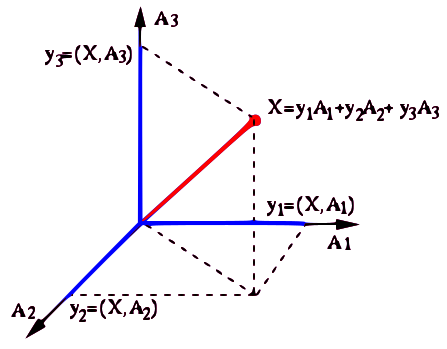
\includegraphics[width=0.7\linewidth]{./img/unitary_transform_1}
\caption[Unitary transform]{Each coefficient (coordinate) $y_i$ is the projection of ${\bf x}$ onto the corresponding basis vector ${\bf a}_i$}
\label{fig:unitary_transform_1}
\end{figure}

As the n-dimensional space can be spanned by the column vectors of \textit{any} $n \times n$ unitary (orthogonal) matrix, a vector  $\bf{x}$ in the space can be represented by any of such matrices, each defining a different transform.\\

\textbf{Examples:}
\begin{itemize}
    \item When $\bf{A} = \mathbf{I} = [\dots, \mathbf{e}_i, \dots]$ is an identity matrix, we have

\end{itemize}





\chapter{Eigenvalue Decomposition}
From: \url{http://fourier.eng.hmc.edu/e176/lectures/algebra/node9.html}\\

For any $n \times n$ square matrix $\mathbf{A}$, if there exists a vector $\mathbf{v}$ such that the following \textit{eigenequation} holds:
\begin{equation}
\mathbf{A}\mathbf{v}=\lambda{}\mathbf{v}
\end{equation}

then $\lambda$ and $\mathbf{v}$ are called the \textit{eigenvalue} and \textit{eigenvector} of matrix $\mathbf{A}$, respectively. In other words, the linear transformation of vector $\mathbf{v}$ by $\mathbf{A}$ has the same effect of scaling the vector by factor $\lambda$. (Note that for an $ n\times n$ non-square matrix $\mathbf{A}$ with $m \neq n$, $\mathbf{A}\mathbf{v}$ is an m-D vector but $\lambda\mathbf{v}$ is an n-D vector, i.e., no eigenvalues and eigenvectors are defined.)\\

Given $\mathbf{A}\mathbf{v}=\lambda\mathbf{v}$, we also have $\mathbf{A}c\mathbf{v}=\lambda{}c\mathbf{v}$ for any scalar constant $c$, i.e., the eigenvector $\mathbf{v}$ is not unique but upt ot any scaling factor. For the uniqueness of $\mathbf{v}$, we typically keep it normalised so that $||v|| = 1$.\\

To obtain $\lambda$, we rewrite the above equation as
\begin{equation}
(\lambda\mathbf{I}-\mathbf{A})\mathbf{v}=0
.\end{equation}

For this homogeneous equation system to have non-zero solutions for $\mathbf{v}$, the determinant of its coefficient matrix has to be zero:
\begin{equation}
\det{(\lambda\mathbf{I}-\mathbf{A})}=|\lambda\mathbf{I}-\mathbf{A}|=0
\end{equation}

This is the \textit{characteristic polynomial equation} of matrix $\mathbf{A}$. Solving this $n^{th}$ order equation of $\lambda$ we get $n$ eigenvalues $\{\lambda_{1},\dots,\lambda_{n}\}$. Substituting each $\lambda{}_{i}$ back into the homogeneous equation system, we get the corresponding eigenvector $\mathbf{v}_{i}$. We can put all $n$ eigen-equations $\mathbf{A}\mathbf{v}_{i}=\lambda{}_{i}\mathbf{v}_{i}$ together and obtain the more compact form:
\begin{equation}
\mathbf{A}\mathbf{V} = \mathbf{A}[\mathbf{v}_{1},\dots,\mathbf{v}_{n}] = [\lambda{}_{1}\mathbf{v}_{1},\dots,\lambda{}_{n}\mathbf{v}_{n}] = 
[\mathbf{v}_{1},\dots,\mathbf{v}_{n}]\begin{bmatrix}
\lambda{}_{1} & 0 & \dots & 0\\
0 & \lambda{}_{2} & \dots & 0\\
\vdots & \vdots & \ddots & \vdots\\
0 & 0 & \dots & \lambda{}_{n}
\end{bmatrix}
= \mathbf{V}\mathbf{\Lambda{}}
\end{equation}

where we have defined
\begin{equation}
\mathbf{\Lambda{}} = \mathit{diag}[\lambda{}_{1},\dots,\lambda{}_{n}] \text{ and } \mathbf{V} = [\mathbf{v}_{1},\dots,\mathbf{v}_{n}]
.\end{equation}

The eigen-equations can be written in some alternative forms:
\begin{equation}
\mathbf{A} = \mathbf{V}\mathbf{\Lambda{}}\mathbf{V}^{-1} \text{ or } \mathbf{V}^{-1}\mathbf{A}\mathbf{V} = \mathbf{\Lambda}
.\end{equation}

In the first form, $\mathbf{A} = \mathbf{A} = \mathbf{V}\mathbf{\Lambda{}}\mathbf{V}^{-1}$ is expressed as a product of three matrices, called \textit{eigenvalue decomposition} of the matrix; in the second form, $\mathbf{A}$ is diagonalized by its eigenvector matrix $\mathbf{V}$ to become a diagonal matrix, its eigenvalue matrix $\mathbf{\Lambda}$.\\

Given $\mathbf{A}\mathbf{v} = \lambda\mathbf{v}$, we have the following:
\begin{itemize}
\item $\mathbf{A}^{T}$ has the same eigenvalues and eigenvectors as $\mathbf{A}$.\\

\textbf{Proof:} As a matrix $\mathbf{A}$ and its transpose $\mathbf{A}^{T}$ have the same determinant, they have the same characteristic polynomial:
\begin{equation}
|\mathbf{A}-\lambda\mathbf{I}| = |(\mathbf{A}-\lambda\mathbf{I})^{T}| = |\mathbf{A}^{T}-\lambda\mathbf{I}|
,\end{equation}

therefore they have the same eigenvalues and eigenvectors.

\item The eigenvalues and eigenvectors of $\mathbf{A}^{*}$ are the complex conjugate of the eigenvalues and eigenvectors of $\mathbf{A}$.

\item $\mathbf{A}^{T}\mathbf{A}$ has the same eigenvectors as $\mathbf{A}$, but its eigenvalues are $\lambda^{2}$.\\

\textbf{Proof:}
\begin{equation}
\mathbf{A}^{T}\mathbf{A}\mathbf{v} = \mathbf{A}^{T}\lambda\mathbf{v} = \lambda^{2}\mathbf{v}
.\end{equation}


\item $\mathbf{A}^{k}$ has the same eigenvectors as $\mathbf{A}$, but its eigenvalues are $\{\lambda_{1}^{k},\dots,\lambda_{n}^{k}\}$, where $k$ is a positive integer.\\

\textbf{Proof:}
\begin{equation}
\mathbf{A}^{2}\mathbf{v} = \mathbf{A}\mathbf{A}\mathbf{v} = \mathbf{A}\lambda\mathbf{v} = \lambda^{2}\mathbf{v}
.\end{equation}

This result can be generalised to
\begin{equation}
\mathbf{A}^{k}\mathbf{v} = \lambda^{k}\mathbf{v}
.\end{equation}

\item In particular when $k = -1$, i.e., the eigenvalues of $\mathbf{A}^{-1}$ are $\{\lambda_{1}^{-1},\dots,\lambda_{n}^{-1}\}$.\\

\textbf{Proof:}\\
Let $\mathbf{\Lambda} = \mathit{diag}(\lambda_{1},\dots,\lambda_{n})$ and $\mathbf{V} = [\mathbf{v}_{1},\dots,\mathbf{v}_{n}]$ be the eigenvalues and eigenvector matrices of a square matrix $\mathbf{A}$:
\begin{equation}
\mathbf{A}\mathbf{V} = \mathbf{\Lambda}\mathbf{V}
\end{equation}

and $\mathbf{\Sigma} = \mathit{diag}(\sigma_{1},\dots,\sigma_{n})$ and $\mathbf{U} = [\mathbf{u}_{1},\dots,\mathbf{u}_{n}]$ be the eigenvalue and eigenvector matrices of $\mathbf{B} = \mathbf{R}^{*}\mathbf{A}\mathbf{R}$, a unitary transform of $\mathbf{A}$:
\begin{equation}
\mathbf{B}\mathbf{U} = (\mathbf{R}^{*}\mathbf{A}\mathbf{R})\mathbf{U} = \mathbf{U}\mathbf{\Sigma}
.\end{equation}

Left multiplying $\mathbf{R}$ on both sides we get the eigenequation of $\mathbf{A}$
\begin{equation}
\mathbf{R}\mathbf{R}^{*}\mathbf{A}\mathbf{R}\mathbf{U} = \mathbf{A}(\mathbf{R}\mathbf{U}) = (\mathbf{R}\mathbf{U})\mathbf{\Sigma}
.\end{equation}

We see that $\mathbf{A}$ and $\mathbf{B} = \mathbf{R}^{*}\mathbf{A}\mathbf{R}$ have the same eigenvalues $\mathbf{\Sigma} = \mathbf{\Lambda}$ and their eigenvector matrices are related by $\mathbf{V} = \mathbf{R}\mathbf{U}$ or $\mathbf{U} = \mathbf{R}^{*}\mathbf{V}$.

\item Given all eigenvalues $\lambda_{1},\dots,\lambda_{n}$ of a matrix $\mathbf{A}$, its trace and determinant can be obtained as
\begin{equation}
\mathit{tr}(\mathbf{A}) = \sum_{k=1}^{n}{\lambda_{k}}
\text{, }
\det(\mathbf{A}) = \prod_{k=1}^{n}{\lambda_{k}}
.\end{equation}

\item The \textit{spectrum} of an $n \times n$ square matrix $\mathbf{A}$ is the set of its eigenvalues $\{\lambda_{1},\dots,\lambda_{n}\}$. The \textit{spectral radius} of $\mathbf{A}$, denoted by $\rho(\mathbf{A})$, is the maximum of the absolute values of the elements in the spectrum:
\begin{equation}
\rho\mathbf{A} = \max{(|\lambda_{1}|,\dots,|\lambda_{n}|)}
,\end{equation}

where $|z| = \sqrt{x^{2}+y^{2}}$ is the modulus of a complex number $z = x+jy$. If all eigenvalues are sorted such that $|\lambda_{1}| \ge \dots \ge |\lambda_{n}|$ then $\rho()\mathbf{A}) = |\lambda_{1}| = |\lambda_{max}|$. As the eigenvalues of $\mathbf{A}^{-1}$ are $\{1/\lambda_{max},\dots,1/\lambda_{min}\}$, $\rho(\mathbf{A}^{-1}) = 1/|\lambda_{min}|$.

\item If $\mathbf{A}$ and $\mathbf{B}$ are similar, i.e.,
\begin{equation}
\mathbf{B} = \mathbf{P}^{-1}\mathbf{A}\mathbf{P}
\end{equation}

then they have the same eigenvalues.\\

\textbf{Proof:}\\

Let $\mathbf{\Lambda}$ and $\mathbf{V}$ be the eigenvalues and eigenvector matrices of $\mathbf{A}$:
\begin{equation}
\mathbf{A}\mathbf{V} = \mathbf{V}\mathbf{\Lambda}
\text{, }
\mathbf{A} = \mathbf{V}\mathbf{\Lambda}\mathbf{V}^{-1}
\end{equation}

then we have
\begin{equation}
\mathbf{B} = \mathbf{P}^{-1}\mathbf{A}\mathbf{P} = \mathbf{P}^{-1}\mathbf{V}\mathbf{\Lambda}\mathbf{V}^{-1}\mathbf{P} = \mathbf{U}\mathbf{\Lambda}\mathbf{U}^{-1}
,\end{equation}

i.e., $\mathbf{\Lambda}$ and $\mathbf{U} = \mathbf{P}^{-1}\mathbf{V}$ are the eigenvalue and eigenvector matrices of $\mathbf{B} = \mathbf{P}^{-1}\mathbf{A}\mathbf{P}$.

\item if $\mathbf{A}$ is Hermitian $\mathbf{A}^{*} = \mathbf{A}^{T} = \mathbf{A}$ (symmetric $\mathbf{A}^{T} = \mathbf{A}$ if real) (e.g., the covariance matrix of a random vector), then all of its eigenvalues $\bar{\lambda}_{i} = \lambda_{i}$ are real, and all of its eigenvectors are orthogonal, $\mathbf{v}_{i}^{*}\mathbf{v}_{j} = 0$ $(i \neq j)$ i.e., $\mathbf{V}^{-1} = \mathbf{V}^{*}$. And we further have
\begin{equation}
\mathbf{A} = \mathbf{V}\mathbf{\Lambda}\mathbf{V}^{-1} = \mathbf{V}\mathbf{\Lambda}\mathbf{V}^{T} = \mathbf{V}\mathbf{\Lambda}^{1/2}\mathbf{\Lambda}^{1/2}\mathbf{V}^{T} = \mathbf{U}\mathbf{U}^{T}
\end{equation}

where $\mathbf{U} = \mathbf{V}\mathbf{\Lambda}^{1/2}$.\\

\textbf{Proof:}\\

Let $\lambda$ and $\mathbf{v}$ be an eigenvalue and the corresponding eigenvector of a Hermitian matrix $\mathbf{A} = \mathbf{A}^{*}$, i.e., $\mathbf{A}\mathbf{v} = \lambda\mathbf{v}$, then we have
\begin{equation}
\begin{array}{ll}
(\mathbf{A}\mathbf{v})^{*}\mathbf{v} & = (\lambda\mathbf{v})^{*}\mathbf{v} = \bar{\lambda}\mathbf{v}^{*}\mathbf{v} = \bar{\lambda}||\mathbf{v}||^{2}\\
& = \mathbf{v}^{*}\mathbf{A}\mathbf{v} = \mathbf{v}^{*}\mathbf{A}^{*}\mathbf{v} = \mathbf{v}^{*}\lambda\mathbf{v} = \lambda||\mathbf{v}||^{2}
\end{array}
\end{equation}

i.e., $\bar{\lambda} = \lambda$ is real. We also have
\begin{equation}
\begin{array}{ll}
\mathbf{v}_{i}^{*}\mathbf{A}\mathbf{v}_{j} & = \mathbf{v}_{i}^{*}\lambda_{j}\mathbf{v}_{j} = \lambda_{j}\mathbf{v}_{i}^{*}\mathbf{v}_{j}\\
& = (\mathbf{v}_{j}^{*}\mathbf{A}\mathbf{v}_{i})^{*} = (\mathbf{v}_{j}^{*}\lambda_{i}\mathbf{v}_{i})^{*} = \bar{\lambda}_{i}\mathbf{v}_{i}^{*}\mathbf{v}_{j} = \lambda_{i}\mathbf{v}_{i}^{*}\mathbf{v}_{j}
\end{array}
\end{equation}

i.e.,
\begin{equation}
\lambda_{j}\mathbf{v}_{i}^{*}\mathbf{v}_{j} = \lambda_{i}\mathbf{v}_{i}^{*}\mathbf{v}_{j}
\text{, or }
(\lambda_{i}-\lambda_{j})\mathbf{v}_{i}^{*}\mathbf{v}_{j} = 0
.\end{equation}

As $\lambda_{i} \neq \lambda_{j}$, we get $\mathbf{v}_{i}^{*}\mathbf{v}_{j} = 0$, i.e., the eigenvectors corresponding to different eigenvalues are orthogonal.\\

When all eigenvectors are normalised $\mathbf{v}_{i}^{*}\mathbf{v}_{i} = ||\mathbf{v}_{i}||^{2} = 1$, they become orthonormal
\begin{equation}
\langle{\mathbf{v}_{i},\mathbf{v}_{j}}\rangle = \mathbf{v}_{i}^{*}\mathbf{v}_{j} = \delta_{ij} = 
\left \{
\begin{array}{ll}
1 & i = j,\\
0 & i \neq j,
\end{array} \right
.\end{equation}

i.e., the eigenvector matrix $\mathbf{V} = [\mathbf{v}_{1}, \dots, \mathbf{v}_{n}]^{T}$ is unitary (orthogonal if $\mathbf{A}$ is real):
\begin{equation}
\mathbf{V}^{-1} = \mathbf{V}^{*}
\text{ i.e. }
\mathbf{V}^{*}\mathbf{V} = \mathbf{I}
\end{equation}

and we have
\begin{equation}
\mathbf{V}^{-1} \mathbf{A} \mathbf{V} = \mathbf{V}^{*} \mathbf{A} \mathbf{V} = \mathbf{\Lambda}
.\end{equation}

Left and right multiplying by $\mathbf{V}$ and $\mathbf{V}^{*} = \mathbf{V}^{-1}$ respectively on the two sides, we get
\begin{equation}
\mathbf{A} = \mathbf{V} \mathbf{\Lambda} \mathbf{V}^{*} =
[\mathbf{v}_{1}, \dots, \mathbf{v}_{n}] \begin{bmatrix}
\lambda_{1} & \dots & 0\\
\vdots & \ddots & \vdots\\
0 & \dots & \lambda_{n}
\end{bmatrix} \begin{bmatrix}
\mathbf{v}_{1}^{*}\\
\vdots\\
\mathbf{v}_{n}^{*}\\
\end{bmatrix} =
\sum_{i=1}^{n}{\lambda_{i} \mathbf{v}_{i} \mathbf{v}_{i}^{*}}
.\end{equation}

This is the \textit{spectral theorem} indicating that $\mathbf{A}$ can be written as a linear combination of $n$ matrices $\mathbf{v}){i} \mathbf{v}_{i}^{*}$ weighted by $\lambda_{i}$ $(i = 1,\dots, n)$.\\

The significance of this property is that a linear operation $\mathbf{y} = \mathbf{A} \mathbf{x}$ applied to vector $\mathbf{x}$ can be mapped to a new vector space in which the operations of the components are independent of each other. Consider
\begin{equation}
\mathbf{y} = \mathbf{A} \mathbf{x} = \mathbf{V} \mathbf{\Lambda} \mathbf{V}^{*} \mathbf{x}
.\end{equation}

Pre-multiplying $\mathbf{V}^{*}$ on both sides we get
\begin{equation}
\mathbf{y}' = \mathbf{V}^{*} \mathbf{y} = \mathbf{\Lambda} \mathbf{V}^{*} \mathbf{x} = \mathbf{\Lambda} \mathbf{x}'
,\end{equation}

where we have defined $\mathbf{x}' = \mathbf{V}^{*} \mathbf{x}$ and $\mathbf{y}' = \mathbf{V}^{*} \mathbf{y}$, the unitary transform of $\mathbf{x}$ and $\mathbf{y}$, respectively. We see that for the ith component we have the following, independent of all other components:
\begin{equation}
y_{i}' = \lambda_{i} x_{i}'
\end{equation}

\item The entries on the diagonal of an upper (or lower) triangular matrix are its eigenvalues.\\

\textbf{Proof:)}\\

Let $\mathbf{A}$ be an upper triangular matrix with $a_{i,j} = 0$ for all $i > j$. The eigenvalues of $\mathbf{A}$ are the roots fo the following homogeneous characteristic equations:
\begin{equation}
\det{(\mathbf{A} - \lambda \mathbf{I})} = \prod_{i=1}^{n}{(a_{ii} - \lambda)} = 0
.\end{equation}

The first equal sign is due to the fact that $\mathbf{A} - \lambda \mathbf{I}$ is also an upper-triangular matrix, and the determinant of an upper-triangular matrix is the product of all its diagonal entries. We therefore see that each diagonal entry $a_{ii}$, as a root of the characteristic equation, is also an eigenvalue of $\mathbf{A}$.

\item Similar matrices have the same eigenvalues.\\

\textbf{Proof:}\\

Let $\lambda$ and $\mathbf{v}$ be an eigenvalue and the corresponding eigenvector of $\mathbf{A}$ satisfying $\mathbf{A} \mathbf{v} = \lambda \mathbf{v}$, and $\mathbf{B} = \mathbf{P}^{-1} \mathbf{A} \mathbf{P}$ be a similar matrix of$\mathbf{A}$. We have $\mathbf{A} = \mathbf{P} \mathbf{B} \mathbf{P}^{-1}$ and
\begin{equation}
\mathbf{A} \mathbf{v} = \mathbf{P} \mathbf{B} \mathbf{P}^{-1} \mathbf{v} = \lambda \mathbf{v}
\text{, i.e., }
\mathbf{B} \mathbf{P}^{-1} \mathbf{v} = \lambda \mathbf{P}^{-1} \mathbf{v}
.\end{equation}

In other words, $\lambda$ is also the eigenvalue of $\mathbf{B}$ with the corresponding eigenvector $\mathbf{P}^{-1} \mathbf{v}$.

\item All eigenvalues of a \textit{stochastic matrix} $\mathbf{P}$ are no greater than 1. A stochastic matrix of which component $P_{ij}$ is the probability for a state transition of a Markov process (chain) from $s_{i}$ to $s_{j}$, i.e. $0 \leq P_{ij} \leq 1$ and $\sum_{j}P_{ij} = 1$.\\

\textbf{Proof: }\\

First, as $\mathbf{P1} = 1$, $\lambda = 1$ is one of the eigenvalues of $\mathbf{P}$. Next let $\lambda$ and $\mathbf{v}$ be an eigenvalue and the corresponding eigenvector of $\mathbf{P}$, i.e., $\mathbf{P} \mathbf{v} = \lambda \mathbf{v}$, and let $|v_{k}| \ge \max\{|v_{1}|, \dots, |v_{n}|\}$. The kth row of the eigenequation is
\begin{equation}
|\lambda v_{k}| \leq |\lambda| |v_{k}| = \left\lvert{\sum_{j=1}^{n}P_{kj}v_{j}}\right\rvert \leq \sum_{j=1}^{n} P_{kj} |v_{j}| \leq  |v_{k}| \sum_{j=1}^{n} P_{kj} = |v_{k}|
\end{equation}

i.e. $|\lambda| \leq 1$.
\end{itemize}

\end{document}
